% \documentclass[]{article}
\documentclass[twocolumn]{article}

\usepackage{geometry}
\geometry{letterpaper, margin=2cm}
\usepackage{amsmath}
\usepackage{graphicx}
\usepackage{subfigure}
\usepackage{cuted}
\usepackage{blindtext}
\usepackage{color}
\usepackage[inline]{showlabels}
\usepackage{showframe}

\usepackage[section]{placeins}
\let\Oldsection\section
\renewcommand{\section}{\FloatBarrier\Oldsection}
\let\Oldsubsection\subsection
\renewcommand{\subsection}{\FloatBarrier\Oldsubsection}
\let\Oldsubsubsection\subsubsection
\renewcommand{\subsubsection}{\FloatBarrier\Oldsubsubsection}

\title{Pure Spin Current Injection in Hydrogenated Graphene Structures}
\author{Reinaldo Zapata-Pe\~na,
Bernardo S. Mendoza,
Anatoli I. Shkrebtii}
\date{}

\begin{document}
\maketitle

\section{Introuction} % (fold)
\label{sec:introuction}

\textcolor{red}{
{\huge Filling with text.}\\
\blindtext
}
\begin{figure}[h]
    \centering
    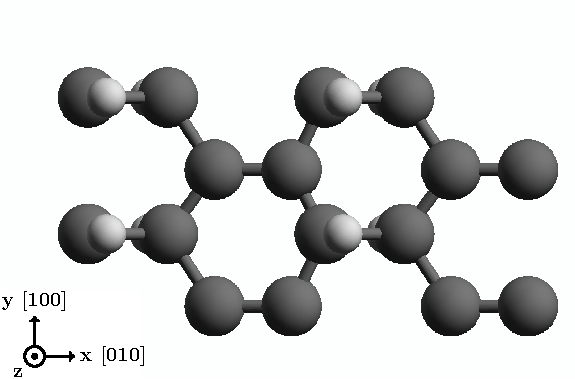
\includegraphics[width=\linewidth]{figures/altstruc1}
    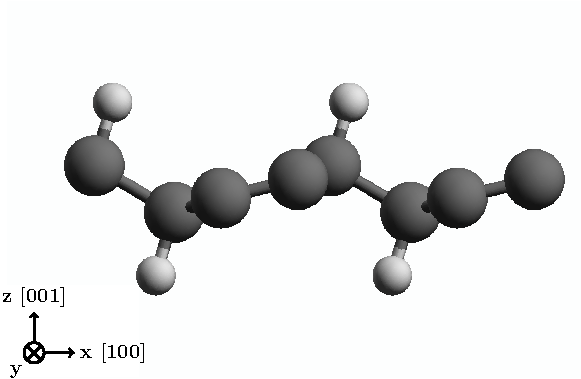
\includegraphics[width=\linewidth]{figures/altstruc2}
    \caption{Alt structure.}
    \label{fig:altstruc}
\end{figure}
\begin{figure}[h!]
    \centering
    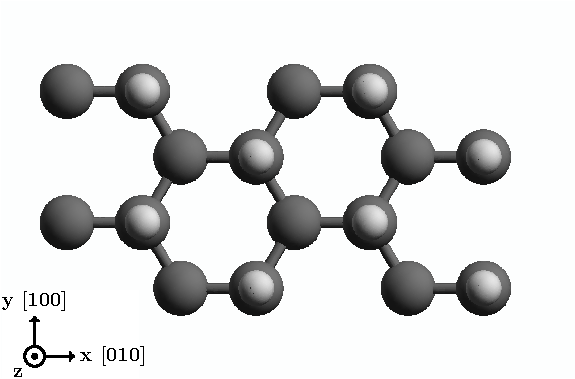
\includegraphics[width=\linewidth]{figures/upstruc1}
    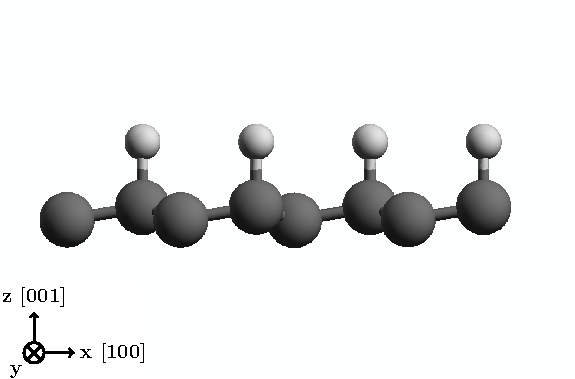
\includegraphics[width=\linewidth]{figures/upstruc2}
    \caption{Up structure}
    \label{fig:upstruc}
\end{figure}
% \begin{figure}[h]
%     \centering
%     \includegraphics[width=\linewidth]{figures/hnbGh-aa-1}
%     \includegraphics[width=\linewidth]{figures/hnbGh-aa-2}
%     \caption{HNBC$_{2}$H-aa structure}
%     \label{fig:aastruc}
% \end{figure}
% \begin{figure}[h]
%     \centering
%     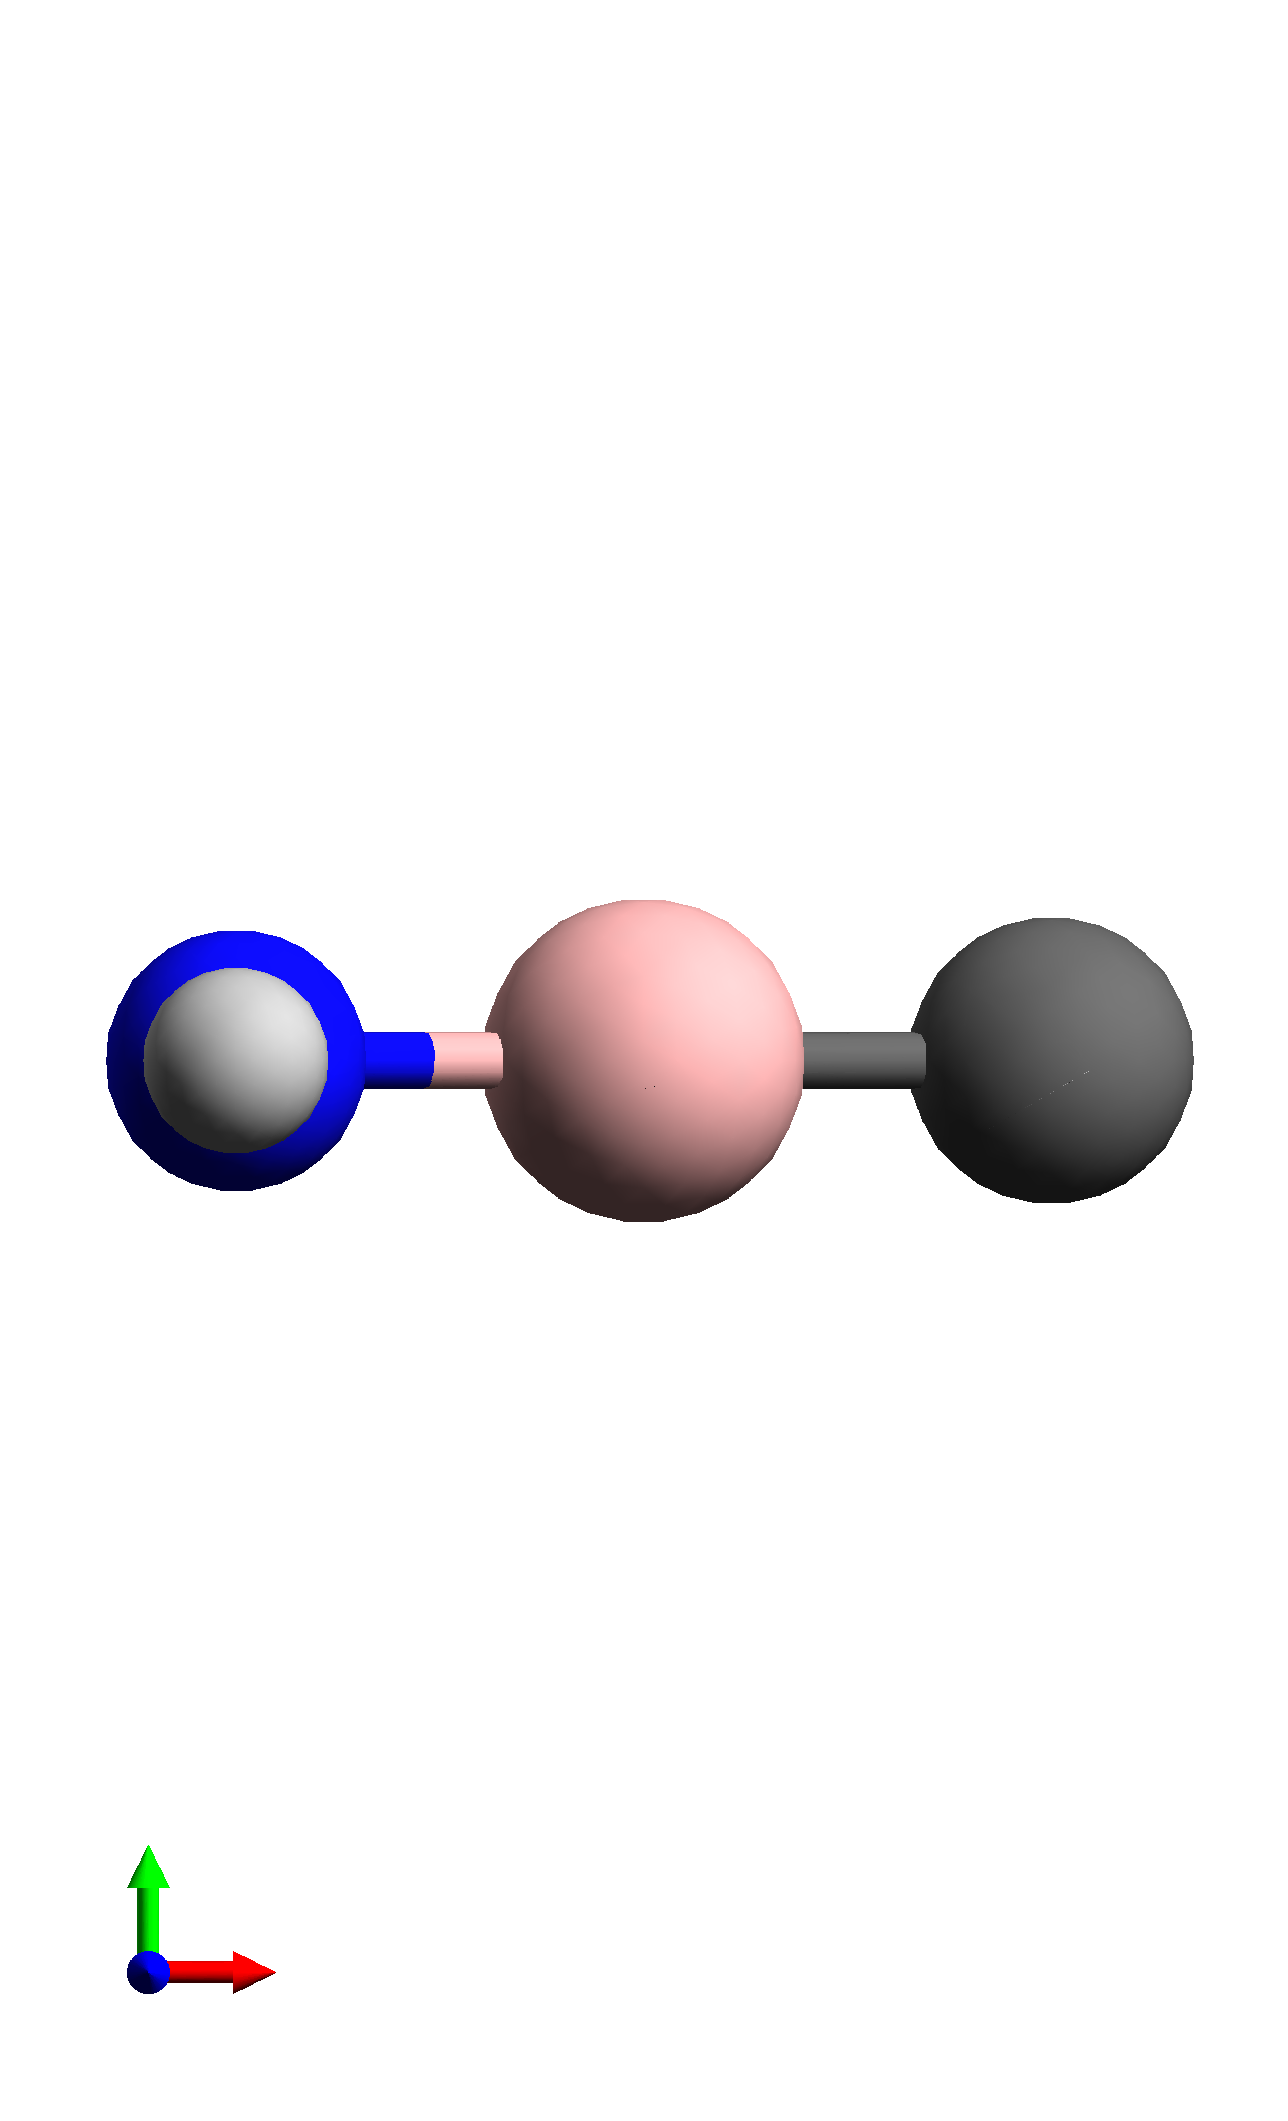
\includegraphics[width=\linewidth]{figures/hnbGh-ab-1}
%     \includegraphics[width=\linewidth]{figures/hnbGh-ab-2}
%     \caption{HNBC$_{2}$H-ab structure}
%     \label{fig:abstruc}
% \end{figure}

% % section introuction (end)
\textcolor{red}{
\blindtext
\blindtext
\blindtext
}

\section{Theory} % (fold)
\label{sec:theory}
The equation for $\mathcal{V}^{\mathrm{ab}}$ for normal incidence in the $xy$
plane with a polarization angle $\alpha$ is given by

\begin{strip}
\begin{align}
\mathcal{V}^{\mathrm{ab}} (\omega) 
&= \frac{\mu^{\mathrm{abxx}}(\omega)
E^{2}(\omega)\cos^{2}(\alpha) + 
\mu^{\mathrm{abyy}}(\omega)
E^{2}(\omega)\sin^{2}(\alpha) + 
2\mu^{\mathrm{abxy}}(\omega)
E^{2}(\omega)\cos(\alpha)\sin(\alpha)}
{\xi^{\mathrm{xx}}(\omega)
E^{2}(\omega)\cos^{2}(\alpha) + 
\xi^{\mathrm{yy}}(\omega)
E^{2}(\omega)\sin^{2}(\alpha)},
\nonumber \\
&= \frac{\mu^{\mathrm{abxx}}(\omega)\cos^{2}(\alpha) + 
\mu^{\mathrm{abyy}}(\omega)\sin^{2}(\alpha) + 
2\mu^{\mathrm{abxy}}(\omega)\cos(\alpha)\sin(\alpha)}
{\xi^{\mathrm{xx}}(\omega)\cos^{2}(\alpha) + 
\xi^{\mathrm{yy}}(\omega)\sin^{2}(\alpha)}.
\label{eq:vab}
\end{align}
\end{strip}

For an angle $\alpha = \frac{\pi}{4}$ this expression can be reduced to 
\begin{align}
\mathcal{V}^{\mathrm{ab}} (\omega)
&= \frac{\mu^{\mathrm{abxx}}(\omega) + \mu^{\mathrm{abyy}}(\omega) + 
2\mu^{\mathrm{abxy}}(\omega)}
{\xi^{\mathrm{xx}}(\omega) + \xi^{\mathrm{yy}}(\omega)}.
\label{eq:vab-90deg}
\end{align}

We also define $|\mathcal{V}^{\mathrm{a}}|$ as 
\begin{equation}\label{eq:vab-mag}
|\mathcal{V}^{\mathrm{a}}| = 
\sqrt {
(\mathcal{V}^{\mathrm{ax}})^{2} +
(\mathcal{V}^{\mathrm{ay}})^{2} +
(\mathcal{V}^{\mathrm{az}})^{2} 
},
\end{equation}
and the corresponding polar and azimuthal angles $\theta$ and $\varphi$ as
\begin{align}
\theta  =& \cos^{-1} \left(  \frac{\mathcal{V}^{\mathrm{az}}}
{|\mathcal{V}^{\mathrm{a}}|} \right),
& 0 \leq &\theta \leq \pi, 
\label{eq:polar-ang} \\
\varphi =& \tan^{-1} \left( \frac{\mathcal{V}^{\mathrm{ay}}}{\mathcal{V}^{\mathrm{ax}}} \right),
& 0 \leq &\varphi \leq 2\pi. \\ 
\label{eq:azimuthal-ang} 
\end{align}

% section theory (end)

\section{Results} % (fold)
\label{sec:results}


We preset the results for $\mathcal{V}^{\mathrm{ab}}$ for the
C$_{16}$H$_{8}$-alt and C$_{16}$H$_{8}$-up structures being both
noncentrosymmetric semi-infinite carbon systems with 50\% hydrogenation in
different arrangements. The \emph{alt} system has alternating hydrogen atoms on
the upper and bottom sides of the carbon sheet, while the \emph{up} system has H
only on the upper side. We take the hexagonal carbon lattice to be on the $xy$
plane for both structures, and the carbon-hydrogen bonds on the perpendicular
$xz$ plane, as depicted in Figs.
\ref{fig:altstruc} and \ref{fig:upstruc}.

Using the ABINIT code \cite{gonzeCPC09} we calculated the self- consistent
ground state and the Kohn-Sham states using density functional theory in the
local density approximation (DFT-LDA) with a planewave basis. We used
Hartwigsen- Goedecker-Hutter (HGH) relativistic separable dual-space Gaussian
pseudopotentials \cite{hartwigsenPRB98} including the spin-orbit interaction for
calculating $\mathcal{V}^{\mathrm{a}}(\omega)$.

The convergence parameters for the calculations of our results corresponding to
the \emph{alt} and \emph{up} structures are cutoff energies of 65\,Ha and
40\,Ha, respectively. The energy eigenvalues and matrix elements were calculated
using 14452 $\mathbf{k}$ points and 8452 $\mathbf{k}$ points in the irreducible
Brillouin zone (IBZ) and present LDA energy band gaps of 0.72\,eV and 0.088\,eV,
respectively for the \emph{alt} and \emph{up} structures. As mentioned in
\cite{zapataPSB2016}, using DFT the LDA is only one method of many other that
can be used to calculate the electronic structure of materials. Also it is known
that all methods predict a different band gap than the obtained in the
experiment. A correction for the band gap energy value can be calculated by
other \emph{ab-initio} methods such as the GW approximation \cite{onidaRMP02}
being this outside the scope of this paper.



\begin{table}[tb]
\center
\begin{tabular}{ccccc}\\
\hline
Layer & Atom & \multicolumn{3}{c}{Position [\AA]} \\
\cline{3-5}
No. & type & $x$ & $y$ & $z$  \\
\hline
1 & H &  -0.61516 &  -1.42140 & \ 1.47237 \\
2 & C &  -0.61516 &  -1.73300 & \ 0.39631 \\
3 & C & \ 0.61516 & \ 1.73300 & \ 0.15807 \\
4 & C & \ 0.61516 & \ 0.42201 &  -0.15814 \\
5 & C &  -0.61516 &  -0.37396 &  -0.39632 \\
6 & H &  -0.61516 &  -0.68566 &  -1.47237 \\
\hline
\end{tabular}
\caption{Unit cell of \emph{alt} structure. Layer division, atom types and
positions for the \emph{alt} structure. The structure unit cell was divided in
six layers corresponding each one to atoms in different $z$ positions.}
\label{tab:altunitcell}
\end{table}

The structures presented here where divided into layers to analyze the he layer-
by-layer contribution for $\mathcal{V}^{\mathrm{ab}}$ response. The \emph{alt}
structure was divided in six layers corresponding the first one to the top
hydrogen atoms, from the second to the forth to carbon atoms in different $z$
positions, and the sixth and last one to the bottom hydrogen atoms. The
\emph{up} structure was divided into two layers, the first one comprised by the
top hydrogen atoms and the second by the carbon atoms. The layer divisions and
atom positions for the unit cells are shown in Tables \ref{tab:altunitcell} and
\ref{tab:upunitcell}.

\begin{table}[tb]
\center
\begin{tabular}{ccccc}\\
\hline
Layer & Atom & \multicolumn{3}{c}{Position [\AA]} \\
\cline{3-5}
No. & type & $x$ & $y$ & $z$  \\
\hline
1 & H & -0.61516 & -1.77416 &  0.73196 \\
1 & H &  0.61518 &  0.35514 &  0.73175 \\
2 & C & -0.61516 & -1.77264 & -0.49138 \\
2 & C & -0.61516 & -0.35600 & -0.72316 \\
2 & C &  0.61516 &  0.35763 & -0.49087 \\
\hline
\end{tabular}
\caption{Unit cell of \emph{up} structure. Layer division, atom types and
positions for the \emph{up} structure. The structure unit cell was divided in
two layers corresponding to hydrogen and carbon atoms.}
\label{tab:upunitcell}
\end{table}



%%%%%%%%%%%%%%%%%%%%%%%%%%%%%%%%%%%%%%%%%%%%%%%%%%%%%%%%%%%%%%%%%%%%%%%%%%%%%%%%
%%%%%%%%%%%%%%%%%%%%%%%%%%%%%%%%%%% ALT %%%%%%%%%%%%%%%%%%%%%%%%%%%%%%%%%%%%%%%%
%%%%%%%%%%%%%%%%%%%%%%%%%%%%%%%%%%%%%%%%%%%%%%%%%%%%%%%%%%%%%%%%%%%%%%%%%%%%%%%%
\subsection{alt} % (fold)
\label{sec:results-alt}

In Fig. \ref{fig:alt-magvxbincang} we present the $\mathcal{V}^{\mathrm{x}}$
spectra resulting from evaluate the Eq. \eqref{eq:vab-mag} at using different
polarization angles $\alpha$ in Eq. \eqref{eq:vab} for the C$_16$H$_8$-alt
structure. The onset of the response is when the energy of the incoming light is
the same of the gap energy. From this picture we can see that for the zone
between the energy range of 0.90\,eV-0.93\,eV and polarization angles between
120$^{\circ}$ and 150$^{\circ}$ is the zone of the maximum response is held
reaching values of $\mathcal{V}^{\mathrm{x}}$ near to 30\,Km/s. Also there is a
second zone between the energy range of 0.70\,eV-0.74\,eV and same polarization
angles where a local maximum of $\mathcal{V}^{\mathrm{x}}$ reaching values near
to 22\,Km/s.We also found that the absolute maximum of the response is obtained
for a polarization angle $\alpha = 145^{\circ}$. The decomposition of
$|\mathcal{V}^{\mathrm{a}}|$ in the corresponding $\mathcal{V}^{\mathrm{x}}$,
$\mathcal{V}^{\mathrm{y}}$, and $\mathcal{V}^{\mathrm{z}}$ components is
depicted in Fig. \ref{fig:alt-vxb}. From this figure we can see that for the
energy range from 0.70\,eV to 0.74\,eV all the $x$, $y$, and $z$ components
contribute with almost the same intensity. In the other hand, for the energy
range from 0.88\,eV to 0.95\,eV there is a major contribution coming from the
$\mathcal{V}^{\mathrm{xz}}$ component.

%%%%%%%%%%%%%%%%%%%%%%%%%%%%% xb [0.6:1.0] %%%%%%%%%%%%%%%%%%%%%%%%%%%%%%%%%%%%%
% \subsubsection{$\mathcal{V}^{\mathrm{x}}$}
\begin{figure}[]
    \centering
    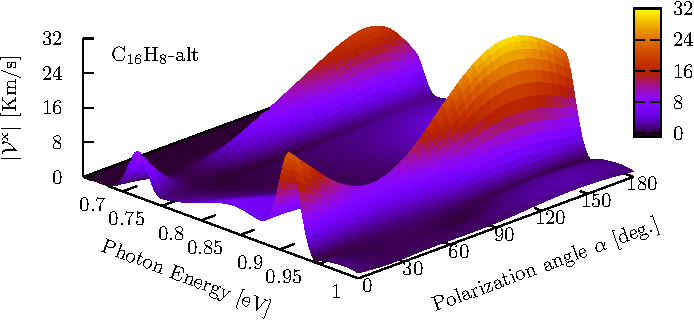
\includegraphics[width=\linewidth]{altplots/alt-magvxb-incang-4545.pdf}
    \caption{$\mathcal{V}^{\mathrm{x}}$ for C$_16$H$_8$-alt structure. The
    maximum response zone is localized for an energy range from 0.90\,eV to
    0.93\,eV. 145$^{\circ}$ and for a polarization angle of the incoming beam from 120$^{\circ}$ to 150$^{\circ}$.}
    \label{fig:alt-magvxbincang}
\end{figure}

\begin{figure}[]
    \centering
    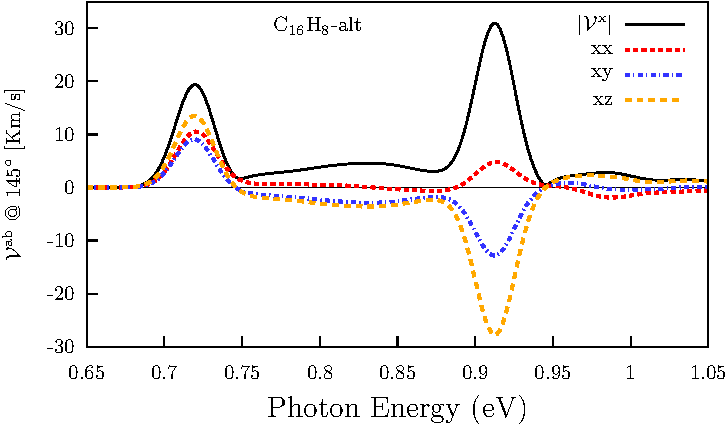
\includegraphics[width=\linewidth]{altplots/alt-vab-xb.pdf}
    \caption{Three components of $\mathcal{V}^{\mathrm{x}} $ @ 145$^{\circ}$.}
    \label{fig:alt-vxb}
\end{figure}


%%%%%%%%%%%%%%%%%%%%%%%%%%%%% yb [0.6:1.0] %%%%%%%%%%%%%%%%%%%%%%%%%%%%%%%%%%%%%
\subsubsection{$\mathcal{V}^{\mathrm{y}}$}
\begin{figure}[ht]
    \centering
    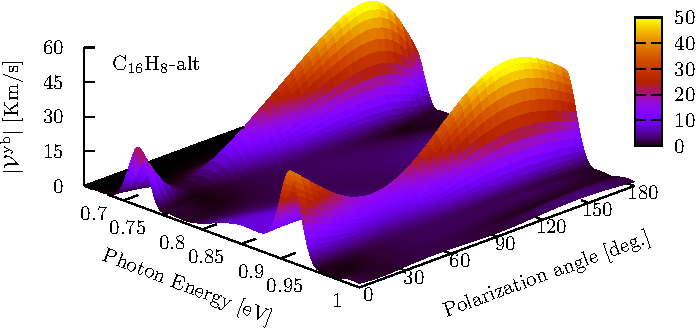
\includegraphics[width=\linewidth]{altplots/alt-magvyb-incang-4545.pdf}
    \caption{The most intense response for $\mathcal{V}^{\mathrm{y}} $ is for 
    145$^{\circ}$.}
    \label{fig:alt-magvybincang1}
\end{figure}
\begin{figure}[ht]
    \centering
    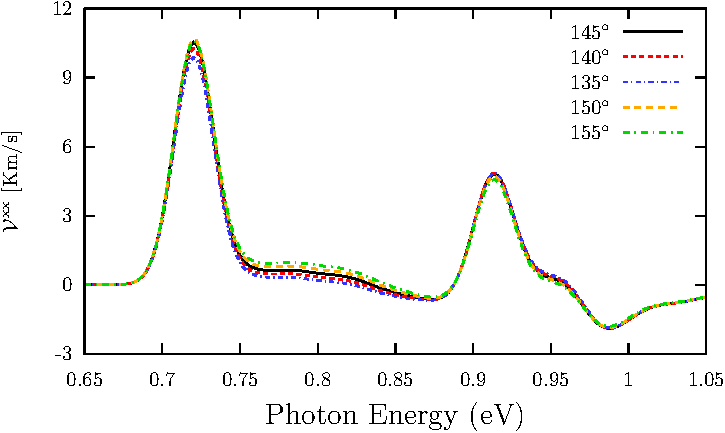
\includegraphics[width=\linewidth]{altplots/alt-vxx.pdf}
    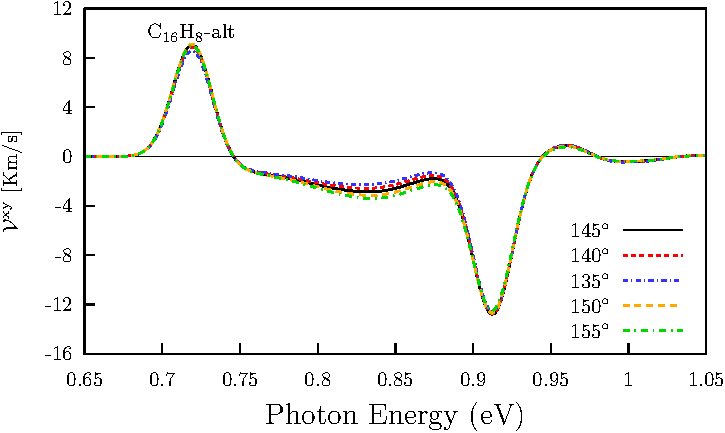
\includegraphics[width=\linewidth]{altplots/alt-vxy.pdf}\\
    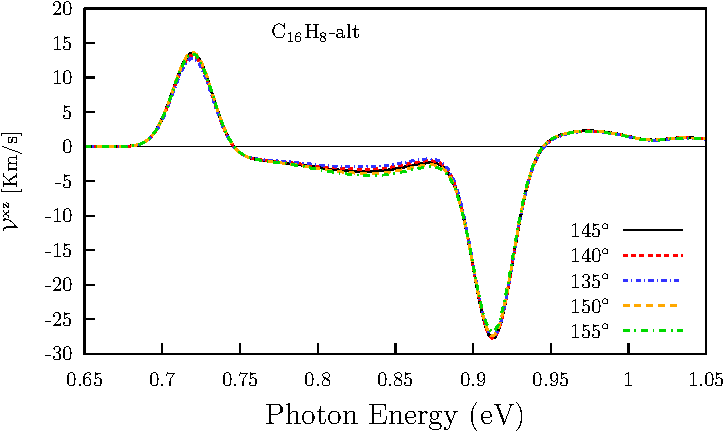
\includegraphics[width=\linewidth]{altplots/alt-vxz.pdf}
    \caption{Cheking angle of incidence for $yb$ components.}
    \label{fig:alt-ybangcomp}
\end{figure}
\begin{figure}[ht]
    \centering
    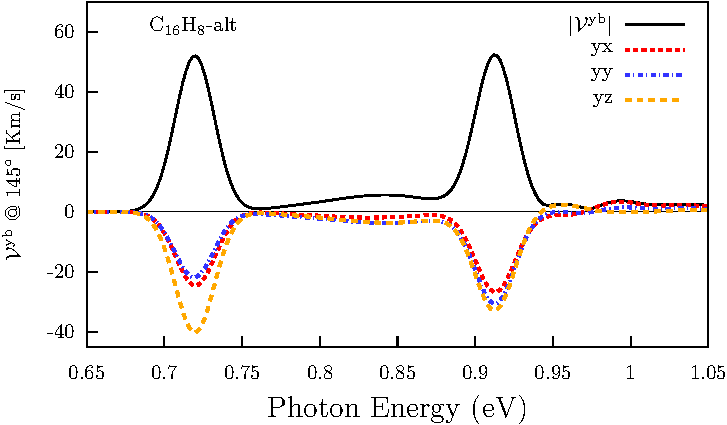
\includegraphics[width=\linewidth]{altplots/alt-vab-yb.pdf}
    \caption{Three components of $\mathcal{V}^{\mathrm{y}} $ @ 145$^{\circ}$.}
    \label{fig:alt-vyb1}
\end{figure}

%%%%%%%%%%%%%%%%%%%%% |V^{ab}| [0.6:1.0] rtp comp %%%%%%%%%%%%%%%%%%%%%%%%%%%%%%
\subsubsection{$|\mathcal{V}^{\mathrm{ab}}|$, angles
$\theta$ and $\varphi$, layers, and comparison with CdSe and GaAs.}
\begin{figure}[ht]
    \centering
    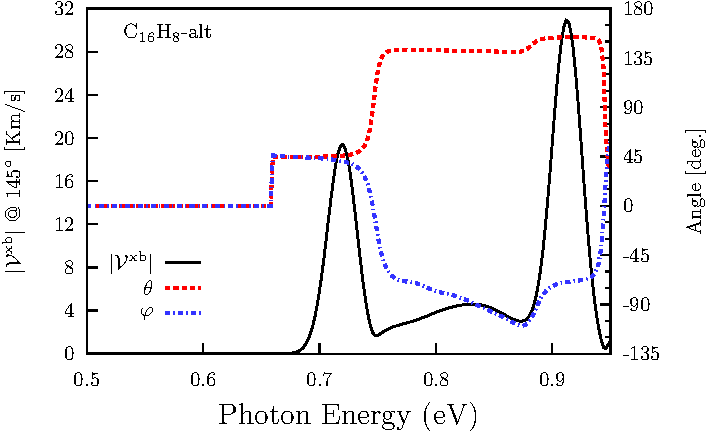
\includegraphics[width=\linewidth]{altplots/alt-vxb-rtp.pdf}
    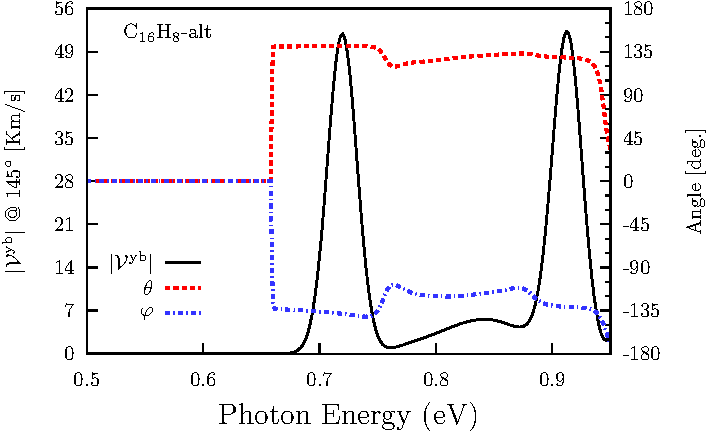
\includegraphics[width=\linewidth]{altplots/alt-vyb-rtp.pdf}
    \caption{$|\mathcal{V}^{\mathrm{ab}}|$ (solid line, leftside scale) and the
    corresponding angles $\theta$ and $\varphi$ (dashed lines, rightside scale).}
    \label{fig:alt-rtp}
\end{figure}

\begin{figure}[ht]
    \centering
    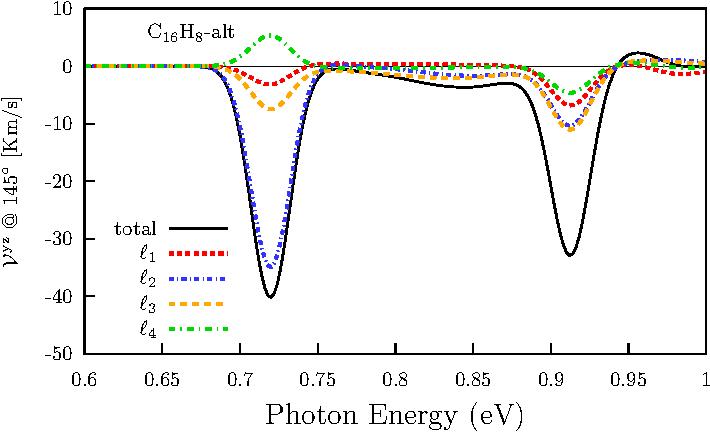
\includegraphics[width=\linewidth]{altplots/alt-vyz-layers.pdf}
    \caption{Layer decomposition for the most intense response:
    $\mathcal{V}^{\mathrm{yz}}$.}
    \label{fig:alt-lay}
\end{figure}

\begin{figure}[ht]
    \centering
    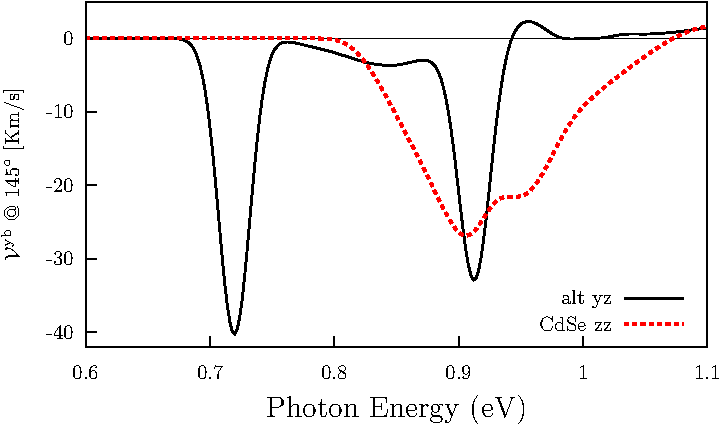
\includegraphics[width=\linewidth]{altplots/alt-vab-comp.pdf}
    \caption{Comparisson of the most intense response vs the most intense
    responses of CdSe and GaAs.}
    \label{fig:alt-comp}
\end{figure}

\begin{figure}[ht]
    \centering
    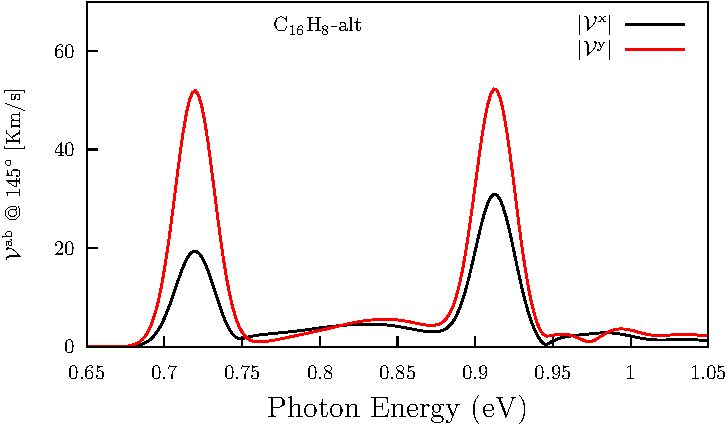
\includegraphics[width=\linewidth]{altplots/alt-absvab.pdf}
    \caption{Comparisson of $|\mathcal{V}^{\mathrm{x}}|$ and $|\mathcal{V}^{\mathrm{y}}|$}    
    \label{fig:alt-xbybcomp}
\end{figure}


% subsection alt (end)


%%%%%%%%%%%%%%%%%%%%%%%%%%%%%%%%%%%%%%%%%%%%%%%%%%%%%%%%%%%%%%%%%%%%%%%%%%%%%%%%
%%%%%%%%%%%%%%%%%%%%%%%%%%%%%%%%%%% UP %%%%%%%%%%%%%%%%%%%%%%%%%%%%%%%%%%%%%%%%%
%%%%%%%%%%%%%%%%%%%%%%%%%%%%%%%%%%%%%%%%%%%%%%%%%%%%%%%%%%%%%%%%%%%%%%%%%%%%%%%%
\subsection{Up (graphone)} % (fold)
\label{sec:results-up}

%%%%%%%%%%%%%%%%%%%%%%%%%%%%% xb [0.0:0.2] %%%%%%%%%%%%%%%%%%%%%%%%%%%%%%%%%%%%%


\subsubsection{$\mathcal{V}^{\mathrm{x}}$ energy range 0.0--0.2 eV }
\begin{figure}[h]
    \centering
    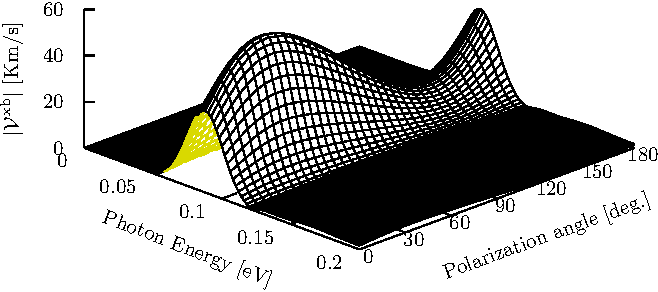
\includegraphics[width=\linewidth]{upplots/up-magvxb-incang-1-4545.pdf}
    \caption{The most intense response for $\mathcal{V}^{\mathrm{x}} $ is for 
    40$^{\circ}$.}
    \label{fig:up-magvxbincang1}
\end{figure}
\begin{figure}[ht]
    \centering
    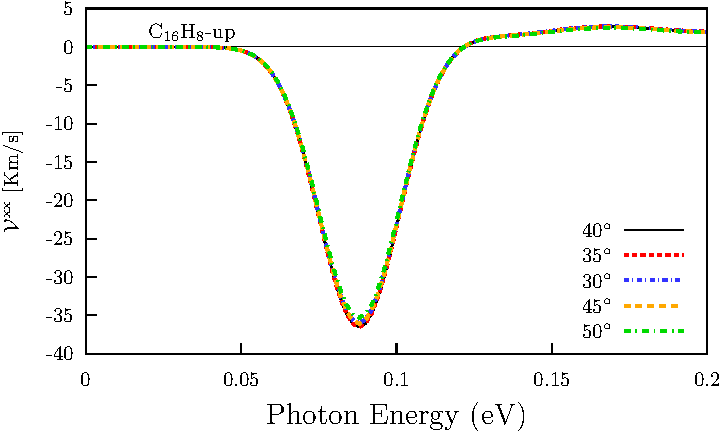
\includegraphics[width=\linewidth]{upplots/up-vab-xx-angcomp.pdf}
    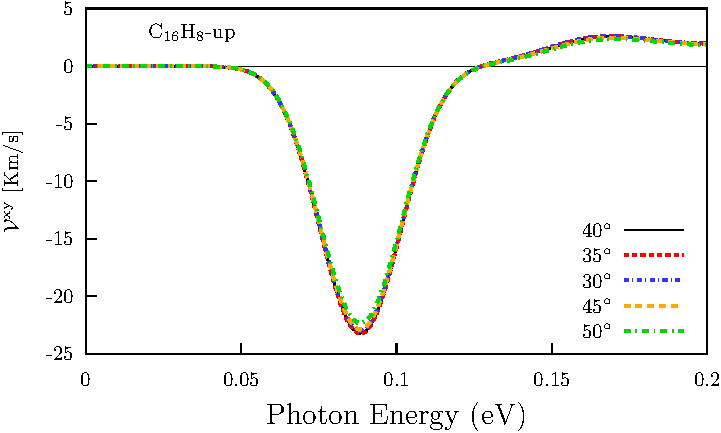
\includegraphics[width=\linewidth]{upplots/up-vab-xy-angcomp.pdf}\\
    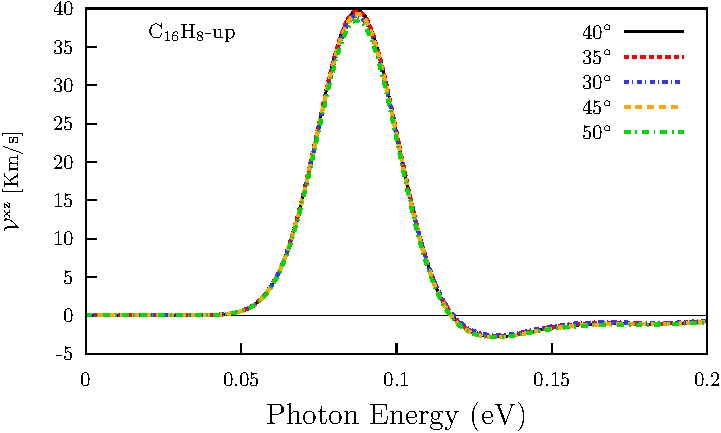
\includegraphics[width=\linewidth]{upplots/up-vab-xz-angcomp.pdf}
    \caption{Cheking angle of incidence for $xb$ components for up structure.}
    \label{fig:up-xbangcomp}
\end{figure}
\begin{figure}[tb]
    \centering
    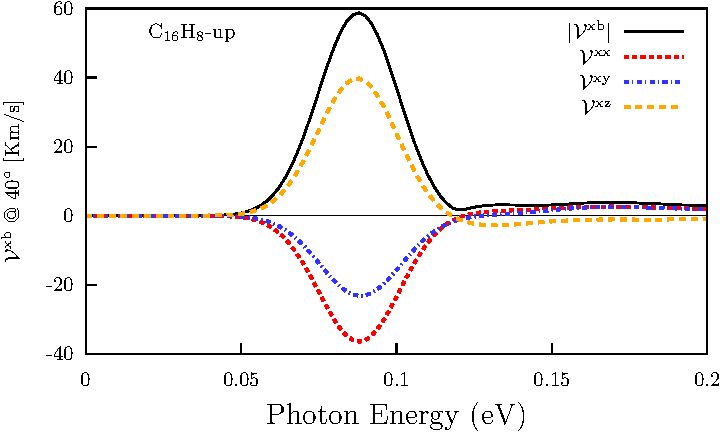
\includegraphics[width=\linewidth]{upplots/up-vab-xb-1.pdf}
    \caption{Three components of $\mathcal{V}^{\mathrm{x}} $ @ 40$^{\circ}$.}
    \label{fig:up-vxb1}
\end{figure}



%%%%%%%%%%%%%%%%%%%%%%%%%%%%% yb [0.0:0.2] %%%%%%%%%%%%%%%%%%%%%%%%%%%%%%%%%%%%%

\subsubsection{$\mathcal{V}^{\mathrm{y}}$ energy range 0.0--0.2 eV }
\begin{figure}[h]
    \centering
    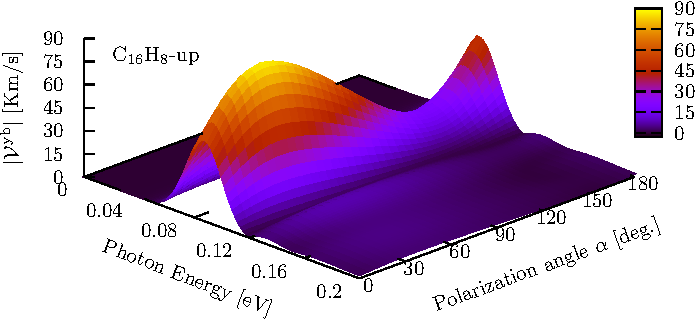
\includegraphics[width=\linewidth]{upplots/up-magvyb-incang-1-4545.pdf}
    \caption{The most intense response for $\mathcal{V}^{\mathrm{y}} $ is for 
    40$^{\circ}$.}
    \label{fig:up-magvybincang1}
\end{figure}
\begin{figure}[ht]
    \centering
    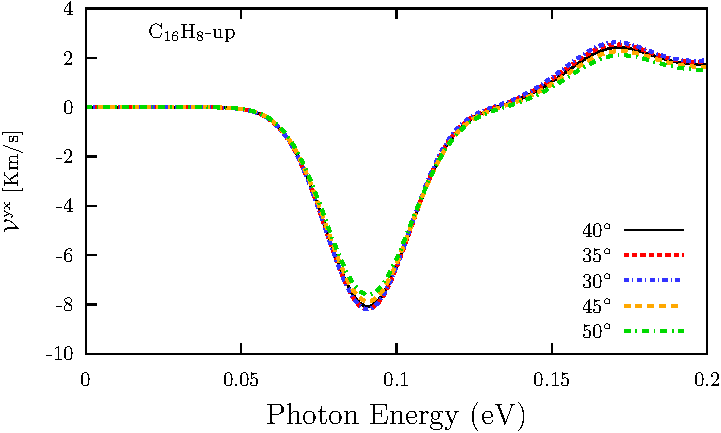
\includegraphics[width=\linewidth]{upplots/up-vab-yx-angcomp.pdf}
    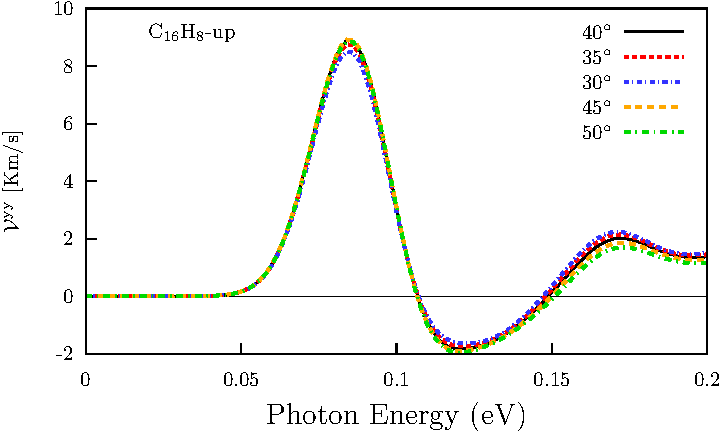
\includegraphics[width=\linewidth]{upplots/up-vab-yy-angcomp.pdf}\\
    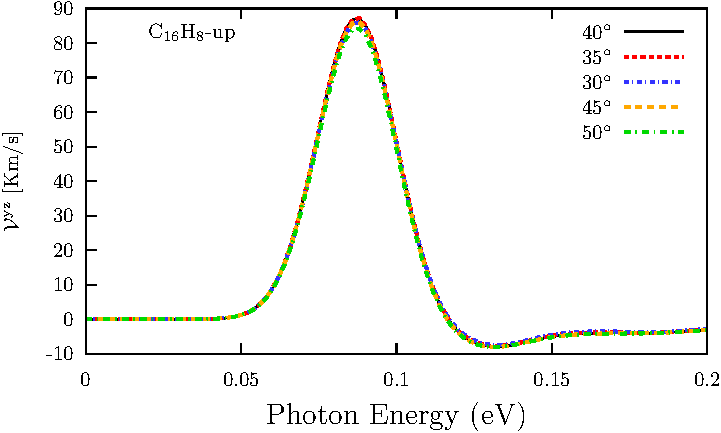
\includegraphics[width=\linewidth]{upplots/up-vab-yz-angcomp.pdf}
    \caption{Cheking angle of incidence for $yb$ components.}
    \label{fig:up-ybangcomp}
\end{figure}
\begin{figure}[ht]
    \centering
    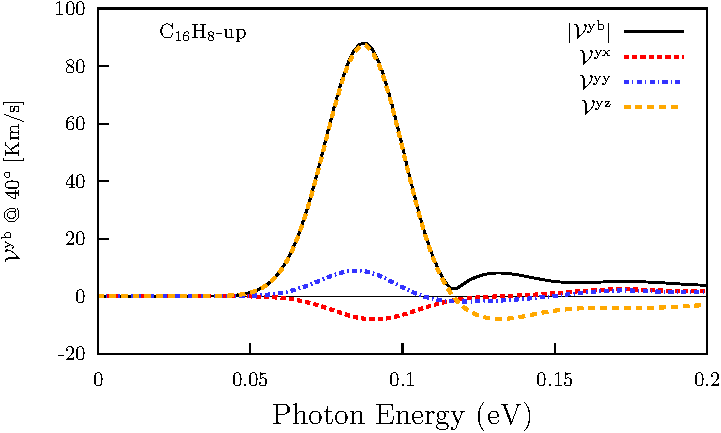
\includegraphics[width=\linewidth]{upplots/up-vab-yb-1.pdf}
    \caption{Three components of $\mathcal{V}^{\mathrm{y}} $ @ 40$^{\circ}$.}
    \label{fig:up-vyb1}
\end{figure}

\begin{figure}[ht]
    \centering
    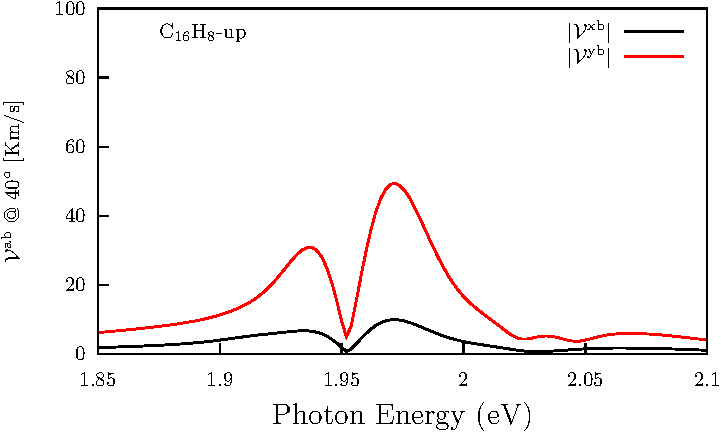
\includegraphics[width=\linewidth]{upplots/up-absvab-1.pdf}
    \caption{Comparisson of $|\mathcal{V}^{\mathrm{x}}|$ and $|\mathcal{V}^{\mathrm{y}}|$}    
    \label{fig:up-xbybcomp-1}
\end{figure}

%%%%%%%%%%%%%%%%%%%%%%%%%%%%% xb [1.8:2.1] %%%%%%%%%%%%%%%%%%%%%%%%%%%%%%%%%%%%%

\subsubsection{$\mathcal{V}^{\mathrm{x}}$ energy range 1.8--2.1 eV }


\begin{figure}[h]
    \centering
    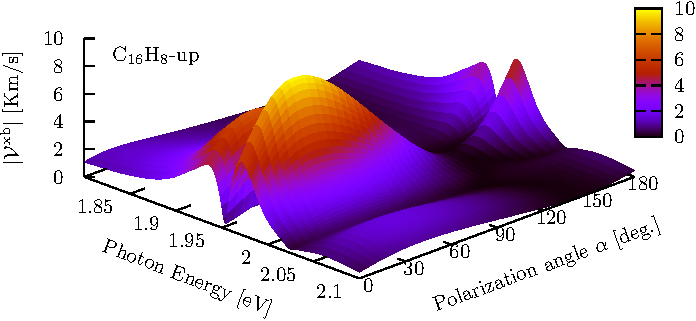
\includegraphics[width=\linewidth]{upplots/up-magvxb-incang-2-4545.pdf}
    \caption{The most intense response for $\mathcal{V}^{\mathrm{x}} $ is for 
    40$^{\circ}$.}
    \label{fig:up-magxbincang2}
\end{figure}
\begin{figure}[h]
    \centering
    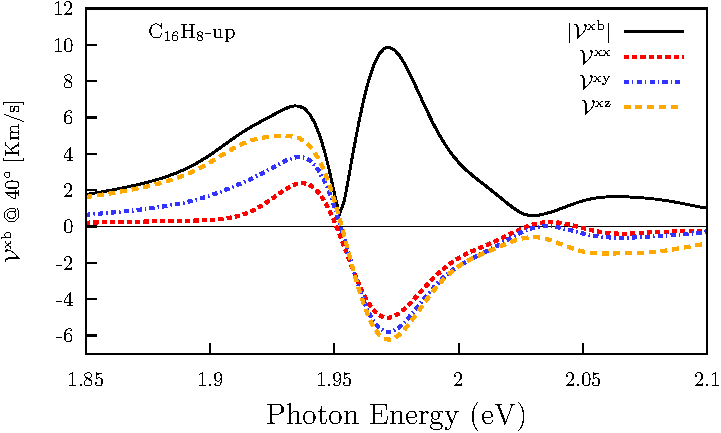
\includegraphics[width=\linewidth]{upplots/up-vab-xb-2.pdf}
    \caption{Three components of $\mathcal{V}^{\mathrm{x}} $ @ 40$^{\circ}$.}
    \label{fig:up-vxb2}
\end{figure}


\begin{figure}[ht]
    \centering
    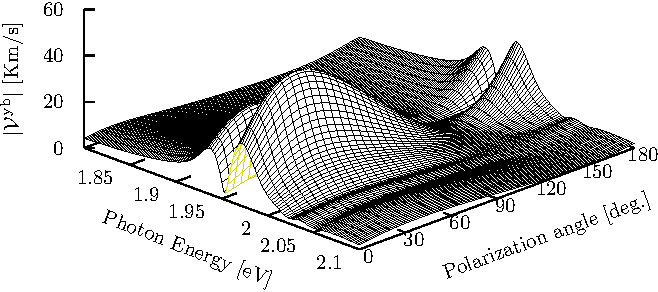
\includegraphics[width=\linewidth]{upplots/up-magvyb-incang-2-4545.pdf}
    \caption{The most intense response for $\mathcal{V}^{\mathrm{y}} $ is for 
    40$^{\circ}$.}
    \label{fig:up-magybincang2}
\end{figure}
\begin{figure}[ht]
    \centering
    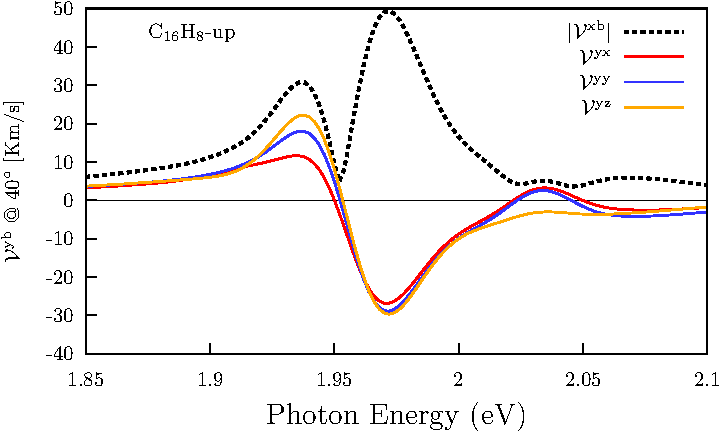
\includegraphics[width=\linewidth]{upplots/up-vab-yb-2.pdf}
    \caption{Three components of $\mathcal{V}^{\mathrm{y}} $ @ 40$^{\circ}$.}
    \label{fig:upvyb2}
\end{figure}

\clearpage

%%%%%%%%%%%%%%%%%%%%% |V^{ab}| [0.0:0.2] rtp comp %%%%%%%%%%%%%%%%%%%%%%%%%%%%%%
\subsubsection{$|\mathcal{V}^{\mathrm{ab}}|$, angles
$\theta$ and $\varphi$, layers, and comparison with CdSe and GaAs for the energy
range of 0.0--0.2 eV.}

\begin{figure}[ht]
    \centering
    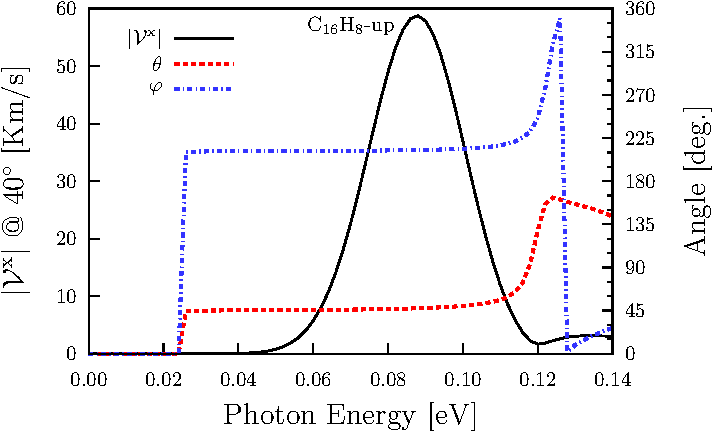
\includegraphics[width=\linewidth]{upplots/up-vxb-rtp-1.pdf}
    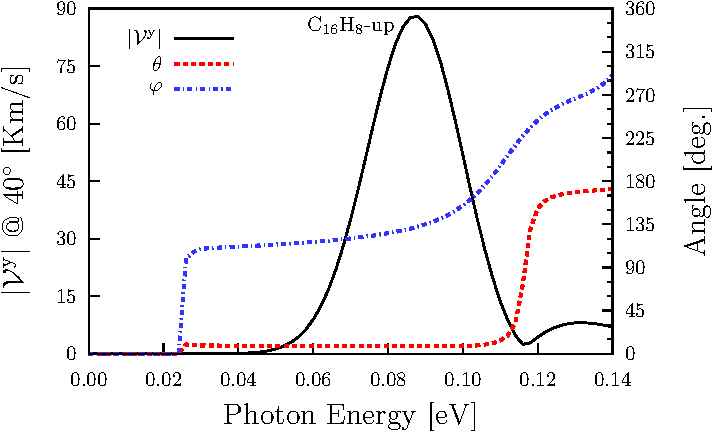
\includegraphics[width=\linewidth]{upplots/up-vyb-rtp-1.pdf}
    \caption{$|\mathcal{V}^{\mathrm{ab}}|$ (solid line, leftside scale) and the
    corresponding angles $\theta$ and $\varphi$ (dashed lines, rightside scale).}
    \label{fig:up-rtp1}
\end{figure}

\begin{figure}[ht]
    \centering
    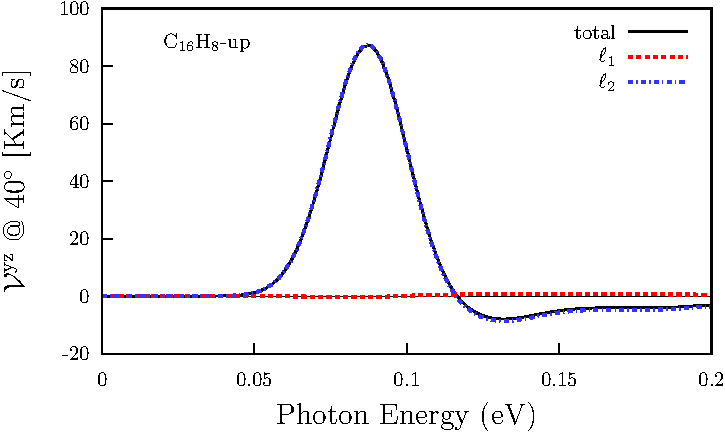
\includegraphics[width=\linewidth]{upplots/up-vyz-layers-1.pdf}
    \caption{Layer decomposition for the most intense response:
    $\mathcal{V}^{\mathrm{yz}}$.}
    \label{fig:up-lay1}
\end{figure}

\begin{figure}[ht]
    \centering
    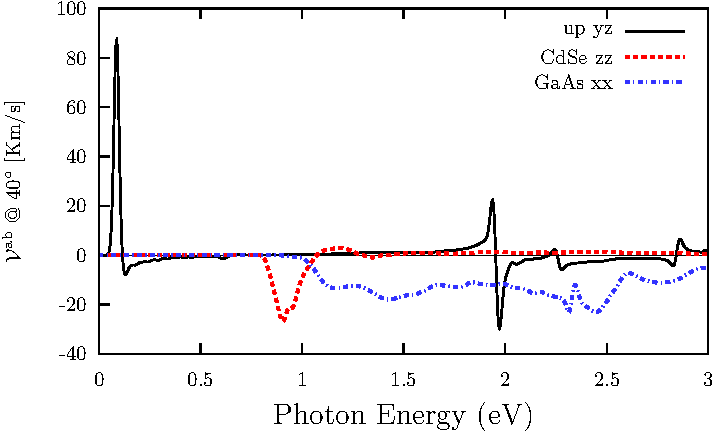
\includegraphics[width=\linewidth]{upplots/up-vab-yz-comp-1.pdf}
    \caption{Comparisson of the most intense response vs the most intense
    responses of CdSe and GaAs.}
    \label{fig:up-comp1}
\end{figure}

%%%%%%%%%%%%%%%%%%%%% |V^{ab}| [1.8:2.1] rtp comp %%%%%%%%%%%%%%%%%%%%%%%%%%%%%%
\subsubsection{$|\mathcal{V}^{\mathrm{ab}}|$, angles
$\theta$ and $\varphi$, layers, and comparison with CdSe and GaAs for the energy
range of 1.8--2.1 eV}

\begin{figure}[ht]
    \centering
    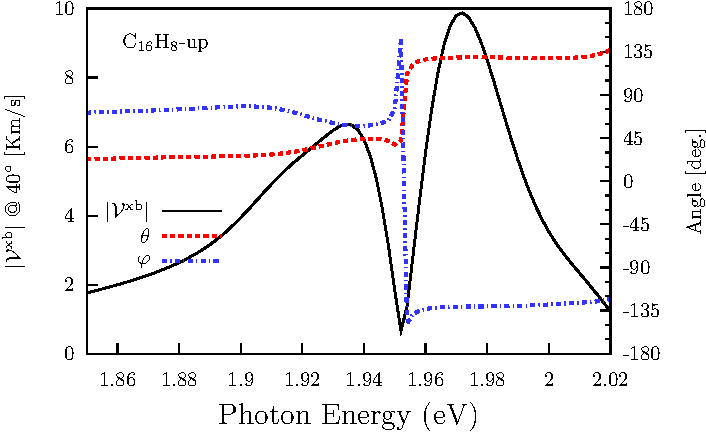
\includegraphics[width=\linewidth]{upplots/up-vxb-rtp-2.pdf}
    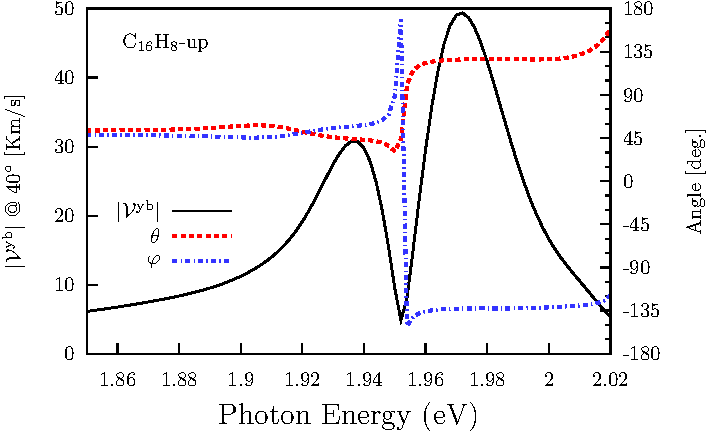
\includegraphics[width=\linewidth]{upplots/up-vyb-rtp-2.pdf}
    \caption{$|\mathcal{V}^{\mathrm{ab}}|$ (solid line, leftside scale) and the
    corresponding angles $\theta$ and $\varphi$ (dashed lines, rightside scale).}
    \label{fig:up-rtp2}
\end{figure}

\begin{figure}[ht]
    \centering
    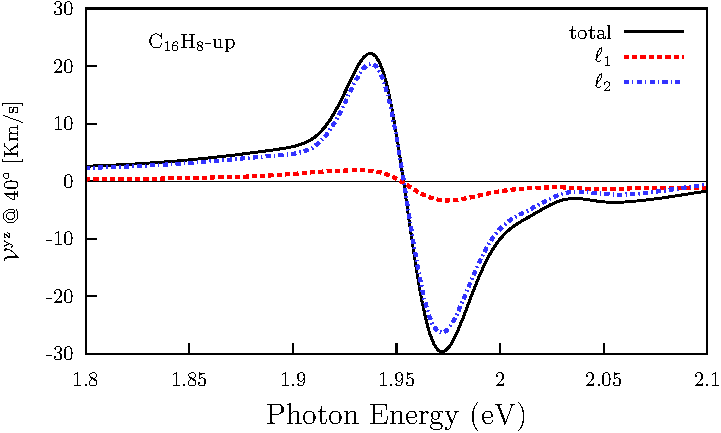
\includegraphics[width=\linewidth]{upplots/up-vyz-layers-2.pdf}
    \caption{Layer decomposition for the most intense response:
    $\mathcal{V}^{\mathrm{yz}}$.}
    \label{fig:up-lay2}
\end{figure}

\begin{figure}[ht]
    \centering
    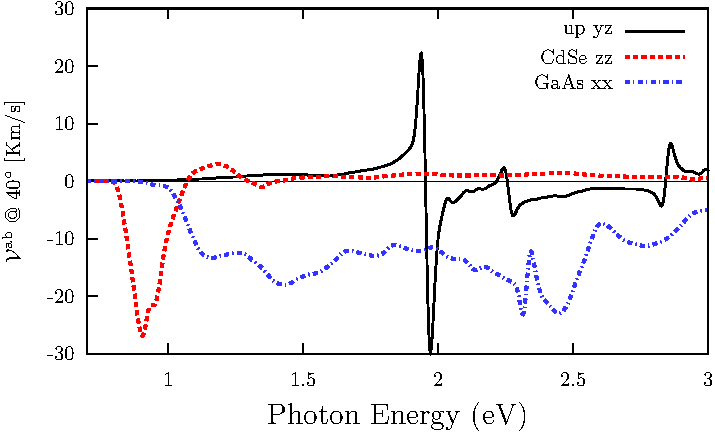
\includegraphics[width=\linewidth]{upplots/up-vab-yz-comp-2.pdf}
    \caption{Comparisson of the most intense response vs the most intense
    responses of CdSe and GaAs.}
    \label{fig:up-comp2}
\end{figure}

\begin{figure}[ht]
    \centering
    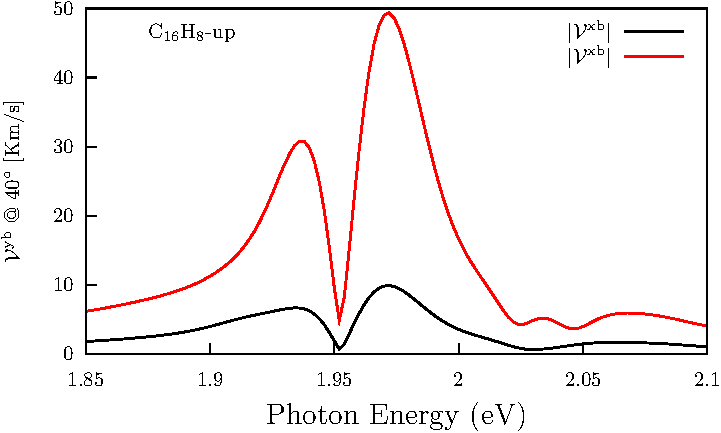
\includegraphics[width=\linewidth]{upplots/up-absvab-2.pdf}
    % \caption{Comparisson of $|\mathcal{V}^{\mathrm{x}}|$ and $|\mathcal{V}^{\mathrm{y}}|$}    
    \label{fig:up-xbybcomp-2}
\end{figure}

% subsection up (end)

% %%%%%%%%%%%%%%%%%%%%%%%%%%%%%%%%%%%%%%%%%%%%%%%%%%%%%%%%%%%%%%%%%%%%%%%%%%%%%%
% %%%%%%%%%%%%%%%%%%%%%%%%%%%%%%%%% AA %%%%%%%%%%%%%%%%%%%%%%%%%%%%%%%%%%%%%%%%%
% %%%%%%%%%%%%%%%%%%%%%%%%%%%%%%%%%%%%%%%%%%%%%%%%%%%%%%%%%%%%%%%%%%%%%%%%%%%%%%

% \subsection{HNBC$_{2}$H-aa} % (fold)
% % \label{sec:results-aa}


% %%%%%%%%%%%%%%%%%%%%%%%%%%% xb [0.5:3.0] %%%%%%%%%%%%%%%%%%%%%%%%%%%%%%%%%%%%%
% \subsubsection{$\mathcal{V}^{\mathrm{x}} $}
% \begin{figure}[ht!]
%     \centering
%     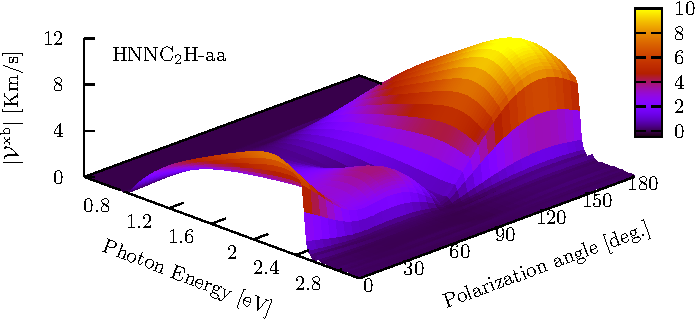
\includegraphics[width=\linewidth]{aaplots/hnbGh-aa-magvxb-incang-4545.pdf}
%     \caption{The most intense response for $\mathcal{V}^{\mathrm{x}} $ is for 
%     155$^{\circ}$.}
%     \label{fig:aa-magvxbincang}
% \end{figure}
% \begin{figure}[ht!]
%     \centering
%     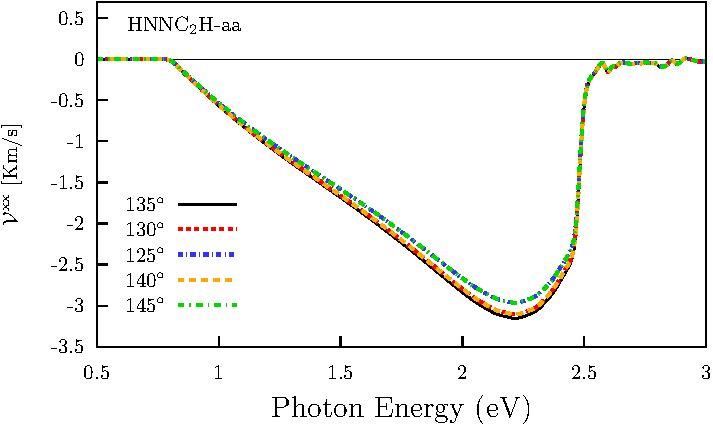
\includegraphics[width=\linewidth]{aaplots/hnbGh-aa-vxx.pdf}
%     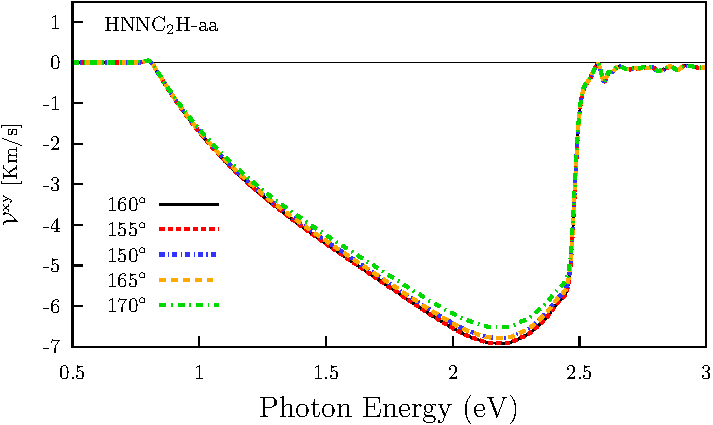
\includegraphics[width=\linewidth]{aaplots/hnbGh-aa-vxy.pdf}\\
%     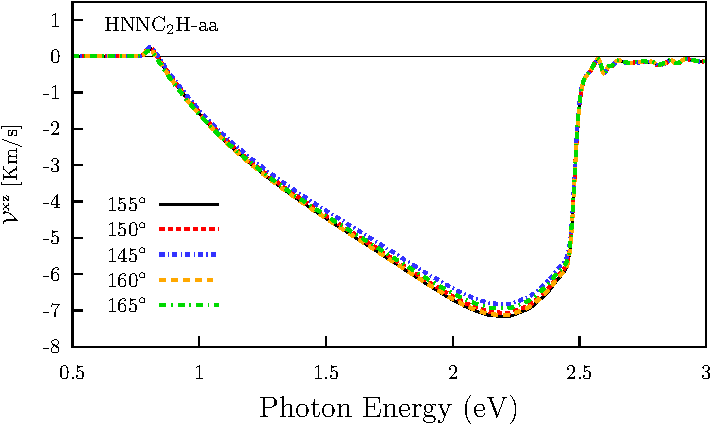
\includegraphics[width=\linewidth]{aaplots/hnbGh-aa-vxz.pdf}
%     \caption{Cheking angle of incidence for $xb$ components. There is a
%     different angle for each component to have the most intense response.}
%     \label{fig:aa-xbangcomp}
% \end{figure}
% \begin{figure}[ht!]
%     \centering
%     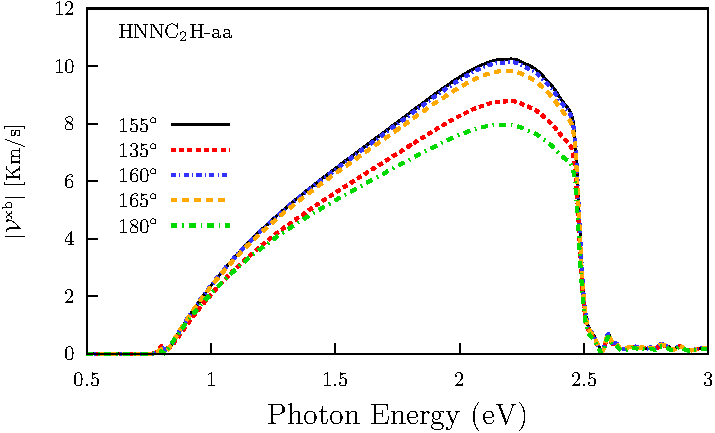
\includegraphics[width=\linewidth]{aaplots/hnbGh-aa-magvxb.pdf}
%     \caption{Comparisson of $|\mathcal{V}^{\mathrm{x}}|$ for different
%     polarization angles.}
%     \label{fig:aa-magvxb}
% \end{figure}
% \begin{figure}[ht!]
%     \centering
%     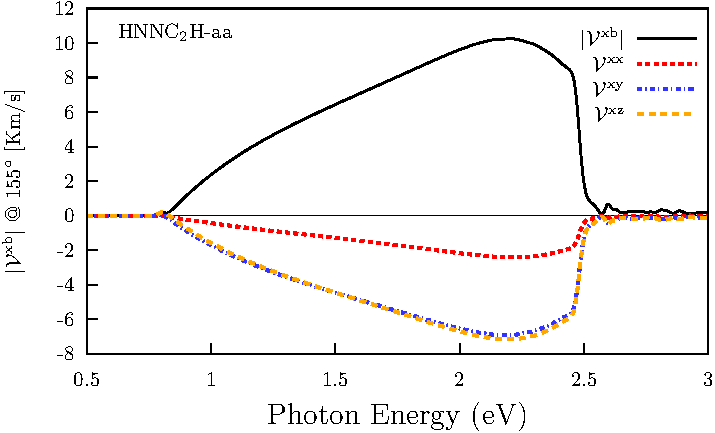
\includegraphics[width=\linewidth]{aaplots/hnbGh-aa-vxb-1.pdf}
%     \caption{Three components of $\mathcal{V}^{\mathrm{x}} $ @ 155$^{\circ}$.}
%     \label{fig:aa-vxb1}
% \end{figure}

% \clearpage

% %%%%%%%%%%%%%%%%%%%%%%%%%%% yb [0.5:3.0] %%%%%%%%%%%%%%%%%%%%%%%%%%%%%%%%%%%%%
% \subsubsection{$\mathcal{V}^{\mathrm{y}} $}
% \begin{figure}[h!]
%     \centering
%     \includegraphics[width=\linewidth]{aaplots/hnbGh-aa-magvyb-incang-4545.pdf}
%     \caption{The most intense response for $\mathcal{V}^{\mathrm{y}} $ is for 
%     155$^{\circ}$.}
%     \label{fig:aa-magvybincang}
% \end{figure}
% \begin{figure}[h!]
%     \centering
%     \includegraphics[width=\linewidth]{aaplots/hnbGh-aa-vyx.pdf}
%     \includegraphics[width=\linewidth]{aaplots/hnbGh-aa-vyy.pdf}\\
%     \includegraphics[width=\linewidth]{aaplots/hnbGh-aa-vyz.pdf}
%     \caption{Cheking angle of incidence for $yb$ components. There is a
%     different angle for each component to have the most intense response.}
%     \label{fig:aa-ybangcomp}
% \end{figure}
% \begin{figure}[ht!]
%     \centering
%     \includegraphics[width=\linewidth]{aaplots/hnbGh-aa-magvyb.pdf}
%     \caption{Comparisson of $|\mathcal{V}^{\mathrm{y}}|$ for different
%     polarization angles.}
%     \label{fig:aa-magvyb}
% \end{figure}
% \begin{figure}[t!]
%     \centering
%     \includegraphics[width=\linewidth]{aaplots/hnbGh-aa-vyb-2.pdf}
%     \caption{Three components of $\mathcal{V}^{\mathrm{y}} $ @ 175$^{\circ}$.}
%     \label{fig:aa-vyb2}
% \end{figure}

% \clearpage

% %%%%%%%%%%%%%%%%%%% |V^{ab}| [0.5:3.0] rtp comp %%%%%%%%%%%%%%%%%%%%%%%%%%%%%%
% \subsubsection{$|\mathcal{V}^{\mathrm{ab}}|$, angles
% $\theta$ and $\varphi$, layers, and comparison with CdSe and GaAs.}
% \begin{figure}[ht]
%     \centering
%     \includegraphics[width=\linewidth]{aaplots/hnbGh-aa-vxb-rtp.pdf}
%     \includegraphics[width=\linewidth]{aaplots/hnbGh-aa-vyb-rtp.pdf}
%     \caption{$|\mathcal{V}^{\mathrm{ab}}|$ (solid line, leftside scale) and the
%     corresponding angles $\theta$ and $\varphi$ (dashed lines, rightside scale).}
%     \label{fig:aa-rtp}
% \end{figure}

% \begin{figure}[ht]
%     \centering
%     \includegraphics[width=\linewidth]{aaplots/hnbGh-aa-vyx-layers.pdf}
%     \caption{Layer decomposition for the most intense response:
%     $\mathcal{V}^{\mathrm{yz}}$.}
%     \label{fig:aa-lay}
% \end{figure}

% \begin{figure}[ht]
%     \centering
%     \includegraphics[width=\linewidth]{aaplots/hnbGh-aa-vab-comp.pdf}
%     \caption{Comparisson of the most intense response vs the most intense
%     responses of CdSe and GaAs.}
%     \label{fig:aa-comp}
% \end{figure}


% \begin{figure}[ht]
%     \centering
%     \includegraphics[width=\linewidth]{aaplots/hnbGh-aa-absvab.pdf}
%     \caption{Comparisson of $|\mathcal{V}^{\mathrm{x}}|$ and $|\mathcal{V}^{\mathrm{y}}|$.}    
%     \label{fig:aa-xbybcomp}
% \end{figure}

% % subsection aa (end)


% %%%%%%%%%%%%%%%%%%%%%%%%%%%%%%%%%%%%%%%%%%%%%%%%%%%%%%%%%%%%%%%%%%%%%%%%%%%%%%
% %%%%%%%%%%%%%%%%%%%%%%%%%%%%%%%%% AB %%%%%%%%%%%%%%%%%%%%%%%%%%%%%%%%%%%%%%%%%
% %%%%%%%%%%%%%%%%%%%%%%%%%%%%%%%%%%%%%%%%%%%%%%%%%%%%%%%%%%%%%%%%%%%%%%%%%%%%%%

% \subsection{HNBC$_{2}$H-ab} % (fold)
% \label{sec:results-ab}

% \begin{figure}[h]
%     \centering
%     \includegraphics[width=\linewidth]{../hnbGh-ab/hnbGh-ab-figures/hnbGh-ab-1}
%     \includegraphics[width=\linewidth]{../hnbGh-ab/hnbGh-ab-figures/hnbGh-ab-2}
%     \caption{HNBC$_{2}$H-ab structure}
%     \label{fig:abstruc}
% \end{figure}

% %%%%%%%%%%%%%%%%%%%%%%%%%%% xb [0.5:3.0] %%%%%%%%%%%%%%%%%%%%%%%%%%%%%%%%%%%%%
% \subsubsection{$\mathcal{V}^{\mathrm{x}} $}
% \begin{figure}[ht!]
%     \centering
%     \includegraphics[width=\linewidth]{abplots/hnbGh-ab-magvxb-incang-4545.pdf}
%     \caption{The most intense response for $\mathcal{V}^{\mathrm{x}} $ is for 
%     155$^{\circ}$.}
%     \label{fig:ab-magvxbincang}
% \end{figure}
% \begin{figure}[ht!]
%     \centering
%     \includegraphics[width=\linewidth]{abplots/hnbGh-ab-vxx.pdf}
%     \includegraphics[width=\linewidth]{abplots/hnbGh-ab-vxy.pdf}\\
%     \includegraphics[width=\linewidth]{abplots/hnbGh-ab-vxz.pdf}
%     \caption{Cheking angle of incidence for $xb$ components. There is a
%     different angle for each component to have the most intense response.}
%     \label{fig:ab-xbangcomp}
% \end{figure}

% \begin{figure}[ht!]
%     \centering
%     \includegraphics[width=\linewidth]{abplots/hnbGh-ab-magvxb.pdf}
%     \caption{Comparisson of $|\mathcal{V}^{\mathrm{x}}|$ for different
%     polarization angles.}
%     \label{fig:ab-magvxb}
% \end{figure}
% \begin{figure}[ht!]
%     \centering
%     \includegraphics[width=\linewidth]{abplots/hnbGh-ab-vxb.pdf}
%     \caption{Three components of $\mathcal{V}^{\mathrm{x}} $ @ 155$^{\circ}$.}
%     \label{fig:ab-vxb}
% \end{figure}

% \clearpage

% %%%%%%%%%%%%%%%%%%%%%%%%%%% yb [0.5:3.0] %%%%%%%%%%%%%%%%%%%%%%%%%%%%%%%%%%%%%
% \subsubsection{$\mathcal{V}^{\mathrm{y}} $}
% \begin{figure}[h!]
%     \centering
%     \includegraphics[width=\linewidth]{abplots/hnbGh-ab-magvyb-incang-4545.pdf}
%     \caption{The most intense response for $\mathcal{V}^{\mathrm{y}} $ is for 
%     155$^{\circ}$.}
%     \label{fig:ab-magvybincang}
% \end{figure}
% \begin{figure}[h!]
%     \centering
%     \includegraphics[width=\linewidth]{abplots/hnbGh-ab-vyx.pdf}
%     \includegraphics[width=\linewidth]{abplots/hnbGh-ab-vyy.pdf}\\
%     \includegraphics[width=\linewidth]{abplots/hnbGh-ab-vyz.pdf}
%     \caption{Cheking angle of incidence for $yb$ components. There is a
%     different angle for each component to have the most intense response.}
%     \label{fig:ab-ybangcomp}
% \end{figure}

% \begin{figure}[ht!]
%     \centering
%     \includegraphics[width=\linewidth]{abplots/hnbGh-ab-magvyb.pdf}
%     \caption{Comparisson of $|\mathcal{V}^{\mathrm{y}}|$ for different
%     polarization angles.}
%     \label{fig:ab-magvyb}
% \end{figure}
% \begin{figure}[ht!]
%     \centering
%     \includegraphics[width=\linewidth]{abplots/hnbGh-ab-vyb.pdf}
%     \caption{Three components of $\mathcal{V}^{\mathrm{y}} $ @ 125$^{\circ}$.}
%     \label{fig:ab-vyb}
% \end{figure}

% \clearpage

% %%%%%%%%%%%%%%%%%%% |V^{ab}| [0.5:3.0] rtp comp %%%%%%%%%%%%%%%%%%%%%%%%%%%%%%
% \subsubsection{$|\mathcal{V}^{\mathrm{ab}}|$, angles
% $\theta$ and $\varphi$, layers, and comparison with CdSe and GaAs.}
% \begin{figure}[ht]
%     \centering
%     \includegraphics[width=\linewidth]{abplots/hnbGh-ab-vxb-rtp.pdf}
%     \includegraphics[width=\linewidth]{abplots/hnbGh-ab-vyb-rtp.pdf}
%     \caption{$|\mathcal{V}^{\mathrm{ab}}|$ (solid line, leftside scale) and the
%     corresponding angles $\theta$ and $\varphi$ (dashed lines, rightside scale).}
%     \label{fig:ab-rtp}
% \end{figure}
 
% % \begin{figure}[ht]
% %     \centering
% %     \includegraphics[width=\linewidth]{}
% %     \caption{Layer decomposition for the most intense response:
% %     $\mathcal{V}^{\mathrm{yz}}$.}
% %     \label{fig:ab-lay}
% % \end{figure}

% \begin{figure}[ht]
%     \centering
%     \includegraphics[width=\linewidth]{abplots/hnbGh-ab-vab-comp.pdf}
%     \caption{Comparisson of the most intense response vs the most intense
%     responses of CdSe and GaAs.}
%     \label{fig:ab-comp}
% \end{figure}


% \begin{figure}[ht]
%     \centering
%     \includegraphics[width=\linewidth]{abplots/hnbGh-absvab.pdf}
%     \caption{Comparisson of $|\mathcal{V}^{\mathrm{x}}|$ and $|\mathcal{V}^{\mathrm{y}}|$.}    
%     \label{fig:ab-xbybcomp}
% \end{figure}

% % subsection ab (end)

% section results (end)

\bibliographystyle{plain}
\bibliography{article.bib}


\end{document}












